\documentclass[11pt]{article}

\usepackage[spanish,activeacute]{babel}
\usepackage{titlesec}
\usepackage{graphicx}
\usepackage{float}
\usepackage{subfig}
\usepackage{chngcntr}
\usepackage{xcolor}
\usepackage{listofitems}
\usepackage[bottom]{footmisc}
\usepackage[hidelinks]{hyperref}
\usepackage[most]{tcolorbox}
\usepackage{listings}

\lstdefinestyle{mystyle}{
    backgroundcolor=\color{white},   
    commentstyle=\color{light-green},
    keywordstyle=\color{fuchsia-vim},
    numberstyle=\tiny\color{darkgray},
    stringstyle=\color{orange-desert-vim},
    basicstyle=\ttfamily\footnotesize,
    breakatwhitespace=false,         
    breaklines=true,                 
    captionpos=b,                    
    keepspaces=true,                 
    numbers=left,                    
    numbersep=5pt,                  
    showspaces=false,                
    showstringspaces=false,
    showtabs=false,                  
    tabsize=2
}
\lstset{style=mystyle}


\setlength{\parindent}{1.0em}
\setlength{\parskip}{1.0em}
\setlength{\emergencystretch}{5.0em}
\setlength{\belowcaptionskip}{-10pt}
\counterwithin{figure}{section}
\titlespacing*{\section}{0em}{3.5em}{1.5em}
\setcounter{tocdepth}{1}
\hypersetup{
	linktoc=all
}


\title{\Huge Software en formato fuente}
\author{Eugenia Damonte, Ariel Fideleff y Mart\'in Go\~ni}
\date{}

\definecolor{fuchsia-vim}{RGB}{168,0,168}
\definecolor{orange-desert-vim}{RGB}{168,87,0}
\definecolor{darkgray}{RGB}{100,100,100}
\definecolor{light-blue}{RGB}{64, 76, 201}
\definecolor{light-red}{RGB}{201, 60, 60}
\definecolor{light-green}{RGB}{65, 181, 104}

\newtcolorbox{code-box}{colback=white!75!gray,colframe=white!15!gray,fontupper=\linespread{1.15}\selectfont}

\newcommand{\codetext}[2]{\large\texttt{\textcolor{#1}{#2}}}
\newcommand{\imagecaption}[1]{\vspace{-7pt}\caption*{\char91\ref{fig:#1}\char93}}


\begin{document}
	\pagenumbering{gobble}
	\maketitle
	\newpage
	\tableofcontents
	\newpage
	\pagenumbering{arabic}
	
	
	\section{Configuraci\'on previa}
		Antes de comenzar a resolver los ejercicios configuramos \texttt{vim} para editar archivos en C. Para hacer esto abrimos el archivo \texttt{\textasciitilde/.vimrc} (en todo caso de no existir, hay que crearlo) que es el archivo de configuraci'on de \texttt{vim}. Estaba vac'io por lo que le a'nad'imos dos l'ineas: \texttt{set nocp} y \texttt{filetype plugin on}. Lo que hace el primer comando es desactivar el modo de compatibilidad. 'Este hace que algunas de las funciones de \texttt{vim} sean deshabilitadas o modificadas para que se comporte de manera similar a \texttt{vi}, el antecesor de \texttt{vim}. La segunda permite utlizar el plugin \texttt{filetype}.
		
		Luego para asegurarnos de tener todos los paquetes de \texttt{vim} utlizamos el comando \texttt{sudo apt-get install vim-gui-common vim-runtime}. El primer paquete tuvo que instalarse y demor'o varios minutos por la velocidad de descarga abismal de los repositorios. El segundo, por el otro lado ya estaba instalado en nuestro caso.
		
		Finalmente creamos el archivo de configuraci'on para los archivos con extensi'on \texttt{.c}, llamado \texttt{c.vim}. Para poder crearlo primero tuvimos que crear la carpeta \texttt{\textasciitilde/.vim/ftplugin}, que es donde se ponen los archivos de configuraci'on. Luego abrimos el mismo con \texttt{vim} y escribimos las configuraciones que quer'iamos usar.
		
		
		\begin{figure}[H]
			\centering
			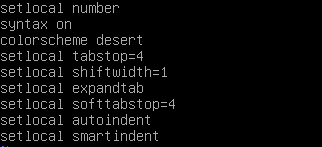
\includegraphics[width=.7\linewidth]{Images/Preamble/Preamble.PNG}
			\caption{Las configuraciones para los archivos \texttt{.c}}
			\label{fig:vim-setup}
		\end{figure}
		
		
	\section{Uso b'asico de gcc}
		Antes de comenzar con el proyecto en s'i, decidimos asegurarnos de que \texttt{gcc} funcionaba correctamente y que sab'iamos usarlo. Para hacer esto copiamos el programa de ejemplo, \texttt{circulo.c}, que se encuentra en el apunte provisto.
		
		\begin{figure}[H]
			\centering
			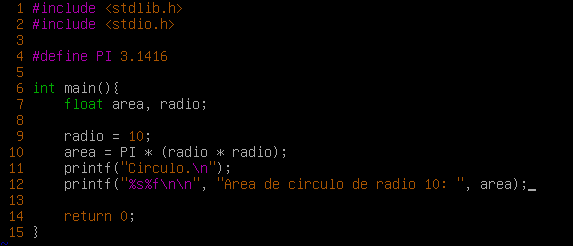
\includegraphics[width=.9\linewidth]{Images/Seccion 1/S1}
			\caption{El programa de ejemplo \texttt{circulo.c}}
			\label{fig:circle-code}
		\end{figure}
		
	\subsection{Compilaci'on directa}
		Una vez copiado el programa realizamos una compilaci'on directa para asegurarnos de que funcionase correctamente. Para hacer esto usamos el comando \texttt{gcc -o circulo circulo.c}. Lo que hace el argumento \texttt{-o} es permitirnos especificar el nombre del archivo de salida, pues si no, el archivo se nombra por defecto \texttt{a.out}.
		
		\begin{figure}[H]
			\centering
			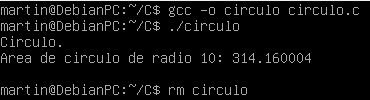
\includegraphics[width=.7\linewidth]{Images/Seccion 1/S1 parte dos}
			\caption{Muestra del funcionamiento de \texttt{circulo.c}}
			\label{fig:basic-compilation}
		\end{figure}
		
	\subsection{Compilaci'on compleja}
		Habiendo comprobado que \texttt{gcc} funcionaba correctamente decidimos intentar compilar el mismo archivo, \texttt{circulo.c}, de manera compleja. Es decir, haciendo cada uno de los pasos que realiza el compilador a la hora de transformar un archivo en C en un programa ejecutable, manualmente uno por uno.
	
	\subsubsection{Preprocesamiento}
		El preprocesado o preprocesamiento es la primera etapa de modificaci'on del c'odigo fuente. Sirve para que, en la fase de compilaci'on, que es la siguiente, el compilador pueda leer correctamente el c'odigo. 
    
    	El trabajo del preprocesador consiste en llevar a cabo las instrucciones dadas por las \textit{directivas} dirigidas al mismo (que, en el caso de C y C++, son las que comienzan con un numeral, como \texttt{\textcolor{fuchsia-vim}{\#define}}, \texttt{\textcolor{fuchsia-vim}{\#include}}, \texttt{\textcolor{fuchsia-vim}{\#ifdef}} y \texttt{\textcolor{fuchsia-vim}{\#error}}, entre otros).

   		En el archivo \texttt{circulo.c} podemos encontrar la directiva  \texttt{\textcolor{fuchsia-vim}{\#define PI} \textcolor{orange-desert-vim}{3.1416}}, que justamente define una constante de nombre \texttt{\textcolor{fuchsia-vim}{PI}} y valor \texttt{\textcolor{orange-desert-vim}{3.1416}}. Esta constante es llamada en la funci'on \texttt{main} de manera que, en vez de escribir  \texttt{\textcolor{orange-desert-vim}{3.1416}}, escribimos simplemente  \texttt{\textcolor{fuchsia-vim}{PI}}.

    	En la figura \ref{fig:preproc_circ},
   		se observa el c'odigo preprocesado que obtuvimos como salida del comando \texttt{gcc -E circulo.c} (tambi'en se puede usar \texttt{cpp circulo.c}, que hace referencia directamente al preprocesador). Si prestamos atenci'on, la directiva antes mencionada no figura en esta salida. Adem'as, en la l'inea que en el c'odigo fuente dec'ia \texttt{\textcolor{darkgray}{area = PI * (radio * radio)}}, ahora dice \texttt{\textcolor{darkgray}{area = \textcolor{orange-desert-vim}{3.1416} * (radio * radio)}}. 

   		En resumen, lo que hizo el preprocesador fue tomar esa definici'on que le indicamos en la directiva y colocar el valor de la constante en las partes del c'odigo en donde se hac'ia referencia a ella.
   		
   		\begin{figure}[H]
   			\centering
			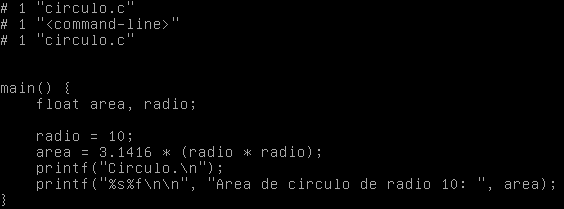
\includegraphics[width=.9\linewidth]{Images/Seccion 1/preprocesado_circulo}
   			\caption{Resultado del preprocesado de \texttt{circulo.c}}
   			\label{fig:preproc_circ}
   		\end{figure}

	\subsubsection{Compilaci'on}
		La compilaci'on es el proceso donde se transforma el c'odigo antes preprocesado (en nuestro caso en C), a assembler propio del procesador de la computadora (en espa'nol, \textit{lenguaje ensamblador}). Para hacer esto usamos el comando \texttt{gcc -S circulo.c}. Notar que directamente nos referimos al archivo con el c'odigo fuente \texttt{circulo.c}, pues el argumento \texttt{-S} ya de por medio realiza el preprocesado antes explicado. Finalmente verificamos que haya funcionado el comando, mostrando las primeras l'ineas del archivo \texttt{circulo.s}, que es donde \texttt{gcc} almacena el compilado.

		\begin{figure}[H]
			\centering
			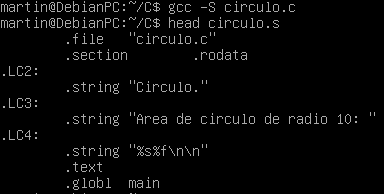
\includegraphics[width=.7\linewidth]{Images/Seccion 1/S1 parte tres.PNG}
			\caption{Primeras 10 l'ineas del resultado de la compilaci'on}
			\label{fig:complex-compilation}
		\end{figure}
		
	\subsubsection{Ensamblado}
		Una vez realizado el compilado, procedemos a ensamblar el archivo. Es decir, transformar el archivo de assembler a c'odigo objeto, un archivo binario en lenguaje m'aquina. Hicimos esto con el comando \texttt{as -o circulo.o circulo.s}. Luego verificamos que haya funcionado revisando qu'e tipo de archivo era \texttt{circulo.o} haciendo uso del comando \texttt{file}.
		
		Otra forma por la cual podr'iamos haber obtenido el archivo en cuesti'on ser'ia utilizando el comando \texttt{gcc -c circulo.c}. Pero, como se puede ver, comenzar'ia a operar directamente desde el c'odigo fuente y realizar'ia todas las etapas previas explicadas.
		
		\begin{figure}[H]
			\centering
			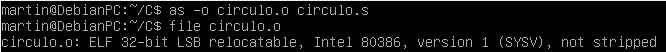
\includegraphics[width=.9\linewidth]{Images/Seccion 1/S1 parte cuatro}
			\caption{Ejecuci'on del ensamblado y detalles del archivo generado}
			\label{fig:complex-assembly}
		\end{figure}
	
		Como el archivo conseguido est'a en lenguaje m'aquina, no podemos verlo con facilidad. En todo caso, podemos hacer uso de un comando como lo es \texttt{objdump -d circulo.o}, que intepreta y permite ver las instrucciones a la computadora contenidas en el archivo. Hay que aclarar que las posiciones de memoria a las que se refiere probablemente no sean correctas, ya que 'estas deben ser relacionadas en el pr'oximo paso, el enlazado, con las librer'ias externas utilizadas.
		
	\subsubsection{Enlazado}
		Finalmente enlazamos el archivo. El enlazado es el proceso mediante el cual se vinculan e incorporan al programa las librer'ias que requiere para poder funcionar. Estas librer'ias est'an compuestas de c'odigo con funciones que uno utiliza en dicho programa. Por ejemplo, en \texttt{circulo.c} usamos funciones como \texttt{\textcolor{darkgray}{printf}}, que hace referencia a la librer'ia \texttt{stdio.h} (t'ipicamente se definir'ia al comienzo del programa de la forma \texttt{\textcolor{fuchsia-vim}{\#include}\textcolor{orange-desert-vim}{\char60stdio.h\char62}} pero, al ser com'unmente utilizado, es incorporado autom'aticamente por el compilador).
		
		En este paso es donde nos encontramos con problemas. El comando que se da en el apunte no funciona. Al usarlo, reporta varios errores: indica que las librer'ias usadas como argumentos no existen y que algunas de las opciones del comando no son v'alidas.
	
		\begin{figure}[H]
			\centering
			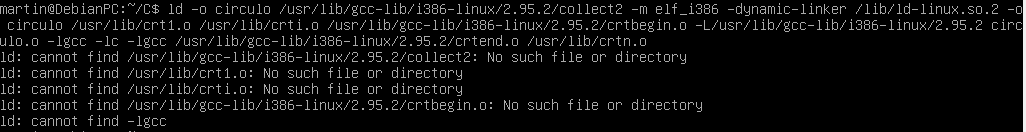
\includegraphics[width=.9\linewidth]{Images/Seccion 1/S1 parte cinco}
			\caption{El primer intento de usar \texttt{ld}, siguiendo el apunte}
			\label{fig:first-ld-attempt}
		\end{figure}
		
		Dado todos los errores que hab'ian, decidimos borrar todas las opciones innecesarias y probar nuevamente. Al hacer esto, los errores anteriores desaparecieron a cambio de uno nuevo. 'Este dec'ia ``\texttt{cannot find entry symbol \textunderscore\/start}'', que se traduce como ``\texttt{no se encuentra el s'imbolo de entrada \textunderscore\/start}''. Luego de algo de investigar descubrimos que este error se debe a que el verdadero punto de entrada\footnotemark\/ de un programa es \texttt{\textunderscore\/start} y no \texttt{main}, siendo que \texttt{\textunderscore\/start} simplemente redirige a 'el. Para solucionar esto, usamos el argumento \texttt{--entry main} que establece a la funci'on \texttt{main} como el punto de entrada del programa.
		
		\footnotetext{El punto de entrada de un programa es donde se ejecutan las primeras instrucciones y se pasa control al programa.}
		
		Una vez hechos estos cambios, la funci'on no dio m'as errores y el programa parec'ia estar listo para usar. A la hora de ejecutarlo, sin embargo, 'este no era reconocido como un programa ejecutable. Para asegurarnos de haber hecho todo correctamente revisamos que el archivo existiese as'i como tambi'en sus permisos, siendo 'estos correctos.
		
		\begin{figure}[H]
			\centering
			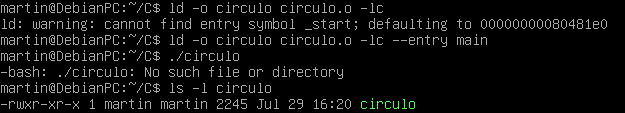
\includegraphics[width=.9\linewidth]{Images/Seccion 1/S1 parte seis}
			\caption{El segundo intento de usar \texttt{ld}}
			\label{fig:second-ld-attempt}
		\end{figure}
		
		Dado que no pod'iamos ejecutar el programa decidimos intentar volver a a'nadir algunas de las opciones que no causaban errores. Primero volvimos a a'nadir las opciones \texttt{-m elf\textunderscore\/i386} y \texttt{--dynamic-linker /lib/ld-linux.so.2}. La primera define el objetivo del compilador\footnotemark\/ y, la segunda, la ubicaci'on del enlazador din'amico\footnotemark\/ a usar.
		
		\footnotetext{El objetivo del compilador es lo que determina que tipo de c'odigo objeto debe producir la funci'on.}
		\footnotetext{Un enlazador din'amico o \textit{dynamic linker} es una forma de enlazar los archivos binarios que se necesitan para que el programa funcione. En este caso, el c'odigo de las funciones se mantiene en la biblioteca y, a la hora de ejecutar el programa, se carga en memoria.}
		
		Luego de hacer estos cambios logramos ejecutar el programa, que parec'ia funcionar correctamente. Sin embargo, al final de 'este tuvimos el error \texttt{Segmentation fault}. Para tratar de averiguar de donde ven'ia el error decidimos debuggear el programa utilizando \texttt{gdb}.
		
		\begin{figure}[H]
			\centering
			\subfloat[Error al correr el programa]{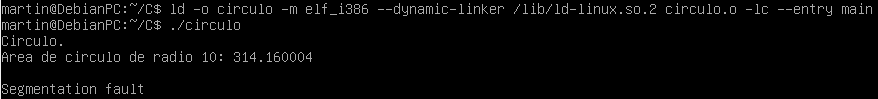
\includegraphics[width=.8\linewidth]{Images/Seccion 1/S1 parte siete}} \par
			\subfloat[Nuestro intento de debuggear el programa]{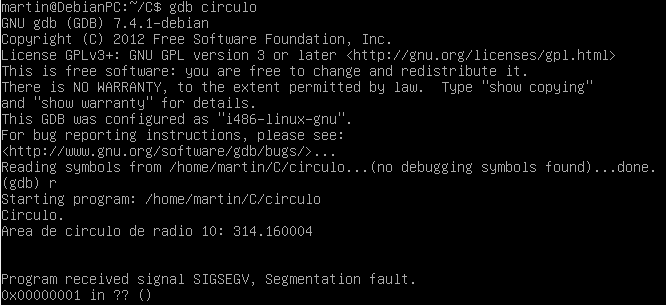
\includegraphics[width=.8\linewidth]{Images/Seccion 1/S1 parte ocho}}
			
			\caption{El tercer intento de usar \texttt{ld}}
			\label{fig:third-ld-attempt}
		\end{figure}
		
		Cuando intentamos debuggear el programa nos encontramos con algo extra'no, y es que \texttt{gdb} no sab'ia de qu'e l'inea proven'ia el error. Esto nos llev'o a creer que proven'ia del enlazado del programa, y no del programa en s'i. Luego de buscar m'as todav'ia, encontramos el problema: nos faltaba incluir las librerias que requer'ia el enlazador din'amico. Para entender por qu'e pasa esto hay que entender c'omo funciona el comando.
		
		Lo primero que hace el comando es especificar la ubicaci'on del enlazador din'amico que requieren las dem'as librerias para acceder a las funciones din'amicas de C. Luego se incluyen otras tres librerias \texttt{/usr/lib/i386-linux-gnu/crt1.o}, \texttt{/usr/lib/i386-linux-gnu/crti.o} y \texttt{/usr/lib/i386-linux-gnu/crtn.o}. La primera es la librer'ia que tiene referencias a los archivos que requiere el enlazador (\texttt{/lib/libc.so.6} y \texttt{/usr/lib/libc\textunderscore\/nonshared.a}). Las otras dos se encargan de que existan \texttt{\textunderscore\/init} y \texttt{\textunderscore\/fini}, que son el c'odigo de inicializaci'on y finalizaci'on. Algo importante de recordar es que la ubicaci'on de las librerias puede cambiar dependiendo del sistema y la instalaci'on especifica. En nuestro caso, las encontramos buscando en \texttt{/usr/lib} y revisando todas las carpetas que parec'ian tener alguna relaci'on.
	
		Es importante notar la posici'on de las librer'ias, \texttt{crti.o} debe ir despu'es de \texttt{crt1.o}. Esto es porque el segundo hace referencia al primero. Adem'as ambas deben ir antes del archivo que se est'a enlazando. Finalmente \texttt{crtn.o} va al final del comando, despu'es de todos los dem'as argumentos.
		
		\begin{figure}[H]
			\centering
			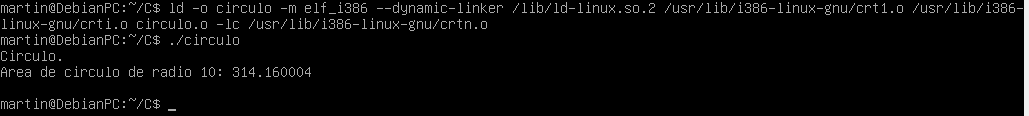
\includegraphics[width=.9\linewidth]{Images/Seccion 1/S1 parte nueve.PNG}
			\caption{El cuarto y 'ultimo intento de usar \texttt{ld}}
			\label{fig:fourth-ld-attempt}
		\end{figure}
		
		Luego de hacer todo esto, el programa finalmente funcion'o y se ejecut'o de manera correcta y sin errores. 

%%%%%%

		Como contamos posteriormente, en el enlazado ``unimos'' todos los c'odigos objetos que forman nuestro programa para crear un 'unico archivo ejecutable. Pero no hay s'olo una forma de enlazar: existe el enlazado est'atico y el din'amico.

		Cuando se usa la primera forma, la parte de la librer'ia que es utilizada en el programa (aunque es probable que alg'un pedazo m'as tambi'en), es copiada en el ejecutable. Es decir, si para crear el ejecutable de \texttt{circulo.c}, a'nadi'eramos la librer'ia \texttt{stdio} de forma est'atica, s'olo la definici'on de \texttt{printf} se copiar'ia, causando que el tama'no del ejecutable aumente. Por otro lado, este tipo de ``linkeo'' es 'util cuando se quiere compartir un archivo ejecutable, pero no sus librer'ias. Es decir, con s'olo enviar dicho archivo, el programa deber'ia funcionar.

		En el enlazado din'amico, las librer'ias no son copiadas en el ejecutable, sino en la memoria RAM. El tama'no del archivo ejecutable no aumenta con respecto al c'odigo objeto del programa, pero s'i ocupa mucho m'as lugar en la memoria RAM que un mismo programa con un enlazado est'atico. 

		Para probar y experimentar las diferencias entre el enlazado din'amico y el est'atico, nos pareci'o una buena idea usar un mismo programa, crear dos ejecutables (uno de cada forma) y compararlos.

		El primer programa con el que hicimos esta prueba fue con \texttt{circulo.c}, que usamos al principio de este trabajo.

		Para enlazarlo din'amicamente, hicimos lo que se muestra previamente en esta secci'on (nombrando al ejecutable como \texttt{circulo\_dinamico}), aunque tambi'en podr'iamos haber usado \texttt{gcc -o circulo\_dinamico circulo.c}, que toma el c'odigo fuente y realiza, adem'as del enlazado, todas las etapas anteriores (preprocesado, compilado y ensamblado).

		Para enlazarlo est'aticamente, usamos un comando parecido al anterior: \texttt{gcc --static -o circulo\_estatico circulo.c}

		Antes de proceder, verificamos que ambos ejecutables funcionaran correctamente (\ref{fig:andan}) y que fueran el tipo de archivo que dese'abamos. Para esto 'ultimo usamos los comandos \texttt{file circulo\_estatico} y \texttt{file circulo\_dinamico}, los resultados pueden verse en la imagen \ref{fig:bien_enlazados}.

		\begin{figure}[H]
			\centering
   			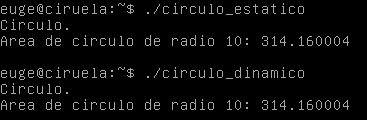
\includegraphics{Images/Seccion 1/ambos_andan.png}
    			\caption{Verificamos que ambos ejecutables anduvieran correctamente.}
    			\label{fig:andan}
		\end{figure}

		\begin{figure}[H]
    			\centering
    			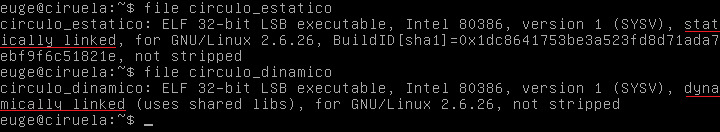
\includegraphics[scale=0.65]{Images/Seccion 1/bien_enlazados_.png}
    			\caption{Verificamos que los ejecutables estuvieran bien enlazados.}
    			\label{fig:bien_enlazados}
		\end{figure}
 
		Lo siguiente que hicimos fue observar la diferencia de tama'no. En la figura \ref{fig:bytes_circulos}, podemos ver la salida del listado con detalle de estos dos ejecutables. La quinta columna indica el tama'no que ocupa cada archivo en bytes. \texttt{circulo\_dinamico}, enlazado din'amicamente, pesa 3649 bytes. Mientras que \texttt{circulo\_estatico}, enlazado est'aticamente, 594184 bytes. Est'a m'as que confirmado que el programa con enlazado est'atico pesa m'as que el din'amico.

% vieron que si quieren poner "de el" tienen que poner "del"? por qué no es lo mismo para "que el"? onda estaría piola decir "quel"

		\begin{figure}[H]
    			\centering
    			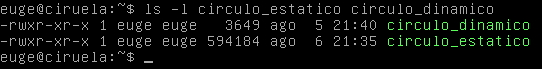
\includegraphics[scale=0.8]{Images/Seccion 1/bytes_circulos.png}
    			\caption{Observamos la diferencia de tama'no entre los ejecutables.}
    			\label{fig:bytes_circulos}
		\end{figure}

		Por 'ultimo, comparamos cu'anta memoria RAM ocupaba la ejecuci'on de cada programa. Sab'iamos que el comando \texttt{ps} % "sabíamos quel comando...", queda mucho mejor
brinda informaci'on variada sobre procesos que se est'an ejecutando en la m'aquina. Pero, como nuestro programa tardaba tan poco en finalizar, no lleg'abamos a verlo en la salida de este.

		Empezamos a investigar sobre distintos programas que sirven para ver datos de un proceso finalizado o de un archivo que tarda muy poco en ejecutarse: time -v, tstime, valgrind... pero no logramos lo que quisimos hasta que recordamos que los procesos detenidos pueden verse en la salida de \texttt{ps}.

		Tratamos de detener la ejecuci'on de alguno de los ejecutables %ejecución de ejecutables, cuánta variedad
de \texttt{circulo.c}, pero ese programa tardaba aproximadamente tres segundos en finalizar y no logr'abamos pararlo. Si consegu'iamos un programa que hiciera m'as cosas (o menos, pero que tuviera un mayor tiempo de ejecuci'on), 'ibamos a poder detener el proceso y cumplir con nuestro objetivo.

		Por suerte ten'iamos hecho un programa con un tiempo de ejecuci'on m'as grande (de aproximadamente doce segundos): \texttt{cosas\_innecesarias.c} \label{cosas_innecesarias} (pueden ver el c'odigo en la secci'on de \texttt{archivos generados}). Hicimos un procedimiento parecido al anterior: creamos dos ejecutables (\texttt{cos\_estaticas} -enlazado est'aticamente- y \texttt{cos\_dinamicas} -enlazado din'amicamente-) y comprobamos que ambos anduvieran.

		\begin{figure}[H]
    			\centering
    			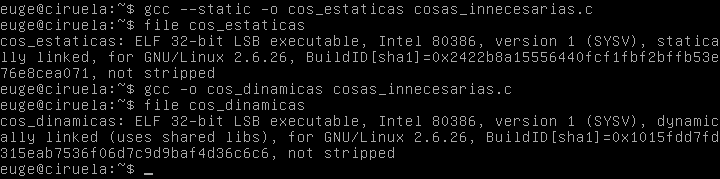
\includegraphics[scale=0.65]{Images/Seccion 1/innecesario.png}
    			\label{fig:innecesario}
		\end{figure}

		Ejecutamos uno de dichos archivos, detuvimos el proceso con la combinaci'on de teclas \texttt{ctrl + Z} y repetimos lo mismo con el otro. Por 'ultimo, hicimos uso del comando \texttt{ps}, de la forma \texttt{ps auxT}. La salida de esa instrucci'on puede observarse en la imagen \ref{fig:ps}

		\begin{figure}[H]
    			\centering
    			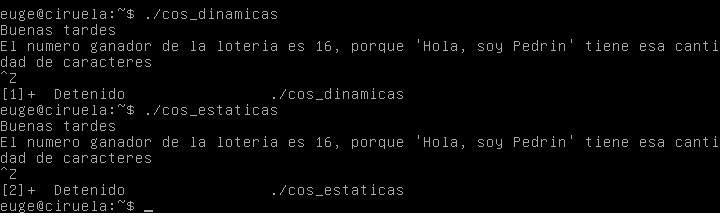
\includegraphics[scale=0.65]{Images/Seccion 1/detenidos.png}
    			\caption{Detuvimos la ejecuci'on de los archivos.}
    			\label{fig:detenidos}
		\end{figure}

		\begin{figure}[H]
    			\centering
    			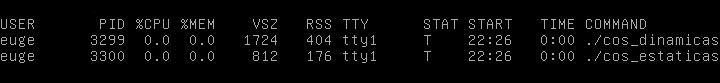
\includegraphics[scale=0.65]{Images/Seccion 1/ps_.png}
    			\caption{Salida del comando \texttt{ps auxT}.}
    			\label{fig:ps}
		\end{figure}

		Como podemos observar, la salida de este comando tiene varios campos: usuario, identificador del proceso, porcentaje del CPU usado, porcentaje de la memoria utilizada, VSZ, RSS, terminal en donde se est'a llevando a cabo el proceso, estado (la ``T'' indica que los procesos est'an detenidos), hora de inicio, tiempo que lleva corriendo, comando que lo inici'o.

		Los campos que nos interesan analizar son VSZ y RSS, relacionados con la memoria RAM. ```VSZ'' representa la ``Virtual Set Size'', que es la memoria RAM que hay disponible para llevar a cabo un proceso. Para calcularla, la m'aquina tiene en cuenta toda la memoria a la que el proceso podr'ia llegar a acceder: la que ocupan las bibliotecas din'amicas y la asignada (memoria que ocupan las variables utilizadas en un programa). %está bien esto?

		\begin{table}[H]
    			\centering
    			\begin{tabular}{|c|}
    			   	\hline VSZ = total\_bibliotecas\_dinamicas + total\_memoria\_asignada \\\hline
		    	\end{tabular}
    			\label{tab:my_label}
		\end{table}

		Por otro lado, la RSS es la memoria RAM que el proceso ya ocup'o. Cuando se calcula se tienen en cuenta la memoria que ocupan las partes de las librer'ias din'amicas que ya fueron cargadas en la RAM y las partes de la memoria asignada que est'a en uso, es decir, s'olo considera los espacios de memoria que tienen valores. %de esto tampoco estoy segura

		\begin{table}[H]
    			\centering
    			\begin{tabular}{|c|}
        			 \hline RSS = bibliotecas\_dinamicas\_cargadas + memoria\_asignada\_usada \\\hline
    			\end{tabular}
    			\label{tab:my_label}
		\end{table}

		Volviendo a la pr'actica: la VSZ de \texttt{cos\_dinamicas} es de 1724 KB, mientras que la de \texttt{cos\_estaticas} es de s'olo 812 KB.
Esta diferencia est'a en las bibliotecas din'amicas: al ser el mismo programa, ambos archivos tienen la misma cantidad de memoria asignada, por lo que, en lo 'unico que pueden diferir es en la memoria que ocupan las bibliotecas din'amicas (que en el caso de \texttt{cos\_estaticas} es igual a cero porque est'a enlazado est'aticamente).  

		Gracias a estos datos, podemos confirmar que, al ser ejecutado, un programa enlazado din'amicamente ocupa m'as memoria RAM que uno con enlazado est'atico.

		Habiendo terminado, decidimos que ya ten'iamos conocimiento suficiente como para intentar compilar un programa usando \texttt{make}.

		
	\section{Uso b'asico de make}
	\subsection{Bases de make}
		El programa \texttt{make} es una herramienta que permite manejar y mantener programas que constan de muchos archivos y tienen m'ultiples dependencias. 'Este evita tener que volver a recompilar el programa manualmente cada vez que se hacen cambios. Autom'aticamente detecta qu'e archivos necesitan ser recompilados y da las instrucciones para hacerlo, todo con un solo comando.
		
		La base del sistema esta un archivo llamado \texttt{makefile}, en el que se almacenan las instrucciones que \texttt{make} utiliza a la hora de compilar un programa. 'Este contiene las reglas de dependencia, macros y las reglas impl'icitas. Las reglas de dependencia son reglas que definen qu'e archivos son necesarios para crear un objetivo\footnotemark. Los macros son variables que almacenan un valor determinado y son muy`utiles para evitar repetir argumentos una gran cantidad de veces. Finalmente, las reglas impl'icitas son una manera de especificar reglas o condiciones usadas a la hora de compilar el programa.
		
		\footnotetext{Un objetivo es el nombre de un archivo(ejecutable o  objeto) o una acci'on de ese \texttt{makefile}.} 

	\subsection{Compilaci'on simple con make}
		Para asegurarnos de que sab'iamos usar \texttt{make}, decidimos compilar el programa de ejemplo que aparece en el apunte, la calculadora con notaci'on polaca. Primero tuvimos que llevar los archivos a la m'aquina virtual, por lo que los descargamos de la p'agina web mencionada en el apunte utilizando \texttt{wget}.
		
		\begin{figure}[H]
				\centering
				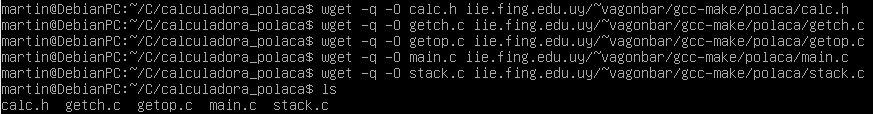
\includegraphics[width=.9\linewidth]{Images/Seccion 2/S2.PNG}
				\caption{Descargamos los archivos a la VM}
				\label{fig:makefile-download}
		\end{figure}
		
		Una vez descargados todos los archivos, compilamos el programa sin utlizar \texttt{make} para asegurarnos de que 'este funcionase correctamente. Para hacer esto usamos \texttt{gcc}, d'andole como argumento todos los archivos que necesitaban ser compilados.
		
		\begin{figure}[H]
				\centering
				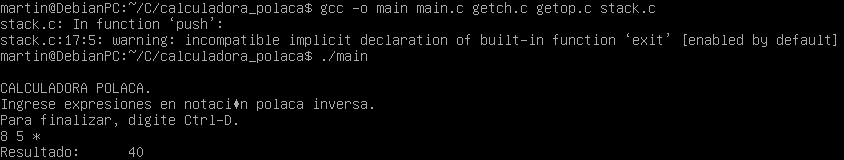
\includegraphics[width=.9\linewidth]{Images/Seccion 2/S2 parte dos.PNG}
				\caption{Compilamos el programa sin \texttt{make}}
				\label{fig:makefile-gcc-compile}
		\end{figure}
	
		Habiendo confirmado que el programa funcionaba, creamos el archivo \texttt{makefile}, necesario para que \texttt{make} funcione. En 'este colocamos todas las reglas necesarias para compilar el programa. 'Estas especificaban qu'e se deb'ia hacer con cada archivo. Para hacer esto usamos reglas de dependencia, las cuales siguen la siguiente estructura:
		
		%Agrande un poco la letra por cuestiones esteticas. Cambienlo si no les parece. --> Lo achiqué un poco y junté un poco las líneas, así no queda tan desproporcionado respecto al resto del texto
		\begin{figure}[H]
			\centering
			\begin{code-box}
				{\large
					\codetext{light-blue}{destino} : \codetext{orange-desert-vim}{dependencias} \vspace{-2pt}
					
					\quad\codetext{light-red}{comando}
				}
			\end{code-box}
		\end{figure} \vspace{-12pt}
		
		Donde \texttt{\textcolor{light-blue}{destino}} es el nombre del archivo a donde ir'a el resultado de las acciones de \texttt{\textcolor{light-red}{comando}}. Es importante notar que \texttt{\textcolor{light-blue}{destino}} tambi'en puede ser una acci'on que puede ser llamada desde el archivo o al usar \texttt{make}. Luego tenemos \texttt{\textcolor{orange-desert-vim}{dependencias}}, que son los archivos que se usan para crear \texttt{\textcolor{light-blue}{destino}} y deben estar presentes en la ubicaci'on especificada. Por 'ultimo, en  \texttt{\textcolor{light-red}{comando}} se indican una o varias instrucciones que son enviadas al shell para ser interpretadas.
		% Pueden tambi'en ser acciones del archivo. % ¿Acciones del archivo?
		
		\begin{figure}[H]
			\centering
			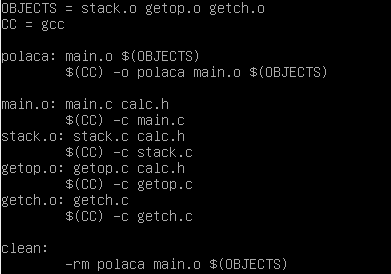
\includegraphics[width=.9\linewidth]{Images/Seccion 2/S2 parte tres.PNG}
			\caption{El \texttt{makefile} creado para compilar el programa}
			\label{fig:makefile}
		\end{figure}
		
		Sabiendo c'omo crear reglas de dependencia y con ayuda del apunte, creamos el \texttt{makefile} necesario para compilar el programa. Tiene adem'as una acci'on para eliminar el archivo ejecutado y todos los archivos \texttt{.o} generados por la compilaci'on.
		
		Usando el comando \texttt{make polaca}, compilamos el programa exitosamente y sin errores. Para verificar que todo funcionase, realizamos la misma operaci'on que hab'iamos utilizado al compilar el programa la primera vez. Al ver que los resultados eran iguales y el programa era ejecutado correctamente, dimos por terminada la pr'actica con \texttt{make}. Antes de pasar a compilar \texttt{w3m}, borramos todos los archivos innecesarios con \texttt{make clean}.
		
		\begin{figure}[H]
			\centering
			\subfloat[Compilamos y ejecutamos el programa]{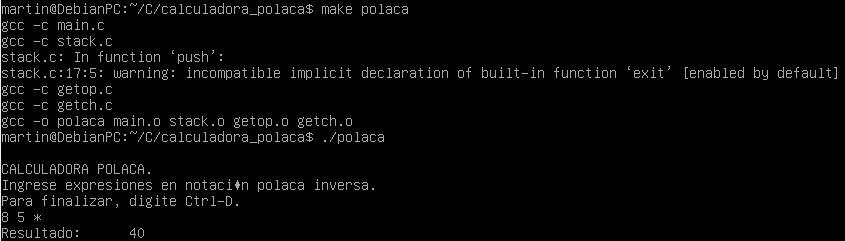
\includegraphics[width=.8\linewidth]{Images/Seccion 2/S2 parte cuatro}} \par
			\subfloat[Borramos todos los archivos innecesarios]{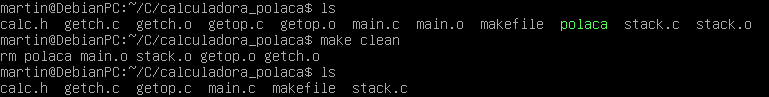
\includegraphics[width=.8\linewidth]{Images/Seccion 2/S2 parte cinco}}
			
			\caption{El comando \texttt{make} en funcionamiento}
			\label{fig:makefile-successful-compile}
		\end{figure}
		
		
	\section{Compilando con make}
	
		Para poder llevar m'as a la pr'actica el conocimiento del funcionamiento de \texttt{make} y la compilaci'on de programas mediante makefiles, decidimos compilar \texttt{w3m}, un navegador web que funciona dentro de la terminal.
		
		Descargamos el c'odigo fuente\footnote{\url{https://sourceforge.net/projects/w3m/files/}}, los archivos necesarios para el proceso, y notamos que se encontraban en un archivo del tipo \texttt{.tar.gz}\footnote{Un archivo \texttt{.tar} es utilizado para almacenar m'ultiples archivos y directorios en un solo archivo. Por otro lado, el sufijo \texttt{.gz}, muestra que los contenidos de dicho archivo se encuentran comprimidos y la forma en que fueron comprimidos.}. Para extraer sus contenidos, usamos el comando \texttt{tar} de linux, aunque para ello primero debimos instalarlo usando \texttt{sudo apt-get install tar}. Hecho esto, el comando que utilizamos fue \texttt{tar -xf w3m-0.5.3.tar.gz}, donde \texttt{-x} implica extraer los archivos, y \texttt{-f} dice que se ejecuten las acciones sobre un archivo cuya ruta se encuentra a continuaci'on de la opci'on. Por el nombre del archivo, es claro que la versi'on de \texttt{w3m} descargada es la \texttt{0.5.3}. Al descomprimir, nos qued'o en el lugar de extracci'on, una carpeta llamada \texttt{w3m-0.5.3} con todos los archivos.
		
		Al abrir la carpeta, vimos la presencia de distintos archivos, entre ellos, pudimos notar algunos de extensi'on \texttt{.c} o \texttt{.h}, que, como sabemos, corresponden a c'odigo hecho en el lenguaje C. Para saber c'omo proceder, nos dirigimos como es habitual al archivo \texttt{README} presente, que dec'ia que deb'iamos dirijirnos a la subcarpeta \texttt{doc} para ver las instrucciones en ingl'es. All'i se encontraba otro \texttt{README} con una breve descripci'on del programa y las instrucciones dichas. Indicaba que primero ejecut'aramos el archivo \texttt{configure}, presente en la carpeta ra'iz, de la forma \texttt{./configure}. Aqu'i empezaron los problemas.
		
		\begin{figure}[H]
			\centering
			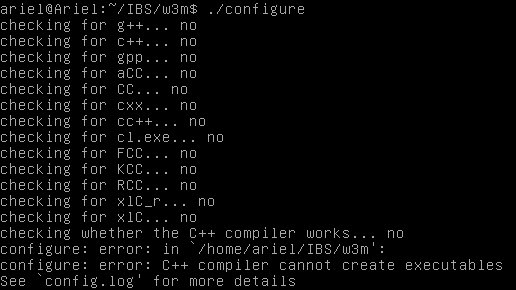
\includegraphics[width=.8\linewidth]{Images/Compile_w3m/g++_missing}
			\caption{Primer intento de ejecuci'on de \texttt{configure}}
			\label{fig:g++_missing}
		\end{figure}
		
		Al ejecutar \texttt{configure}, se report'o el error ``\texttt{C++ compiler cannot create executables}'', es decir, el compilador de C++ no puede crear ejecutables. Tambi'en nos inform'o que para m'as detalles pod'iamos revisar el archivo generado \texttt{config.log}. All'i pudimos ver todo el historial de las acciones realizadas por \texttt{configure}, y notamos que verificaba por la presencia de ciertos programas, que parec'ian ser todos compiladores de C++, implicando que no exist'ia ninguno en la m'aquina.
		
		\begin{figure}[H]
			\centering \captionsetup{justification=centering}
			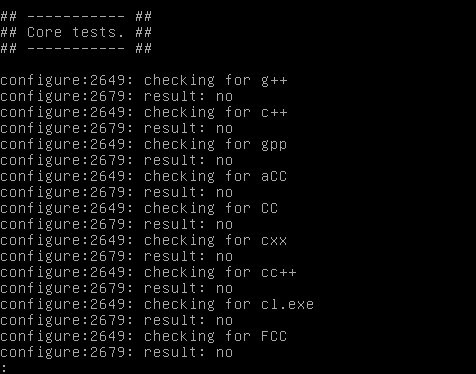
\includegraphics[width=.7\linewidth]{Images/Compile_w3m/g++_missing_log}
			\caption{Contenidos de \texttt{configure.log} luego del primer intento de ejecuci'on de \texttt{configure}}
			\label{fig:g++_missing_log}
		\end{figure}
		
		Instalamos entonces el primero de entre los que probaba, \texttt{g++}, de la forma \texttt{sudo apt-get install g++}. Esta vez, al correr \texttt{configure} pareci'o lograr mayor progreso que en el anterior intento pero, de todas formas, la ejecuci'on presentaba un error: \texttt{configure: error: gc.h not found}.
		
		\begin{figure}[H]
			\centering \captionsetup{justification=centering}
			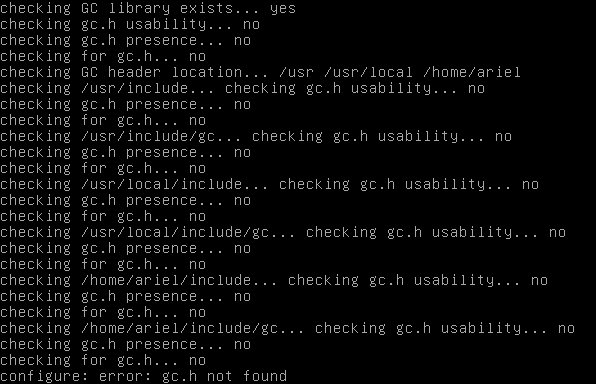
\includegraphics[width=.8\linewidth]{Images/Compile_w3m/gc_missing}
			\caption{Segundo intento de ejecuci'on de \texttt{configure}}
			\label{fig:gc_missing}
		\end{figure}
		
		Estuvimos investigando este problema, viendo c'omo se pod'ia obtener este archivo faltante. Notamos que verificaba por la existencia del archivo mencionado en m'ultiples rutas antes de mostrar el error. Luego de explorar un poco, entendimos que lo que buscaba el programa era algo llamado ``Garbage Collector'', que es lo que usan m'ultiples lenguajes de programaci'on como mecanismo para la gesti'on adecuada de la memoria, y as'i tanto reservar espacios de dicha memoria, liberarlos, tener cuenta del espacio libre y ocupado, e incluso la reorganizaci'on del mismo a fin de liberar el mayor espacio posible que pueda ser utilizado, compactando los espacios de memoria libres entre los ocupados, dejando la mayor cantidad contigua libre posible. 
		
		Despu'es de saltar mucho entre p'aginas buscando, llegamos a una con informaci'on detallada sobre las dependencias que uno puede instalar en Linux, en espec'ifico la de \texttt{libgc-dev}\footnote{\url{https://ubuntu.pkgs.org/16.04/ubuntu-main-amd64/libgc-dev_7.4.2-7.3_amd64.deb.html}} ya que vimos que contiene entre sus archivos, el archivo \texttt{gc.h} faltante. Lo instalamos de la forma \texttt{sudo apt-get install libgc-dev}.
		
		Probamos nuevamente correr \texttt{configure}, y por lo que vimos, pareci'o finalizar sin inconvenientes.
		
		\begin{figure}[H]
			\centering \captionsetup{justification=centering}
			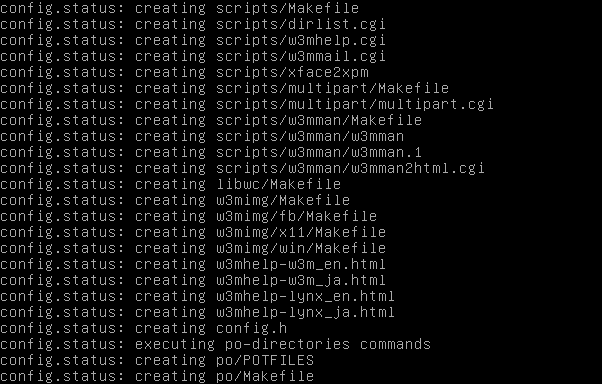
\includegraphics[width=.8\linewidth]{Images/Compile_w3m/configure_successful}
			\caption{Tercer intento (y correcto) de ejecuci'on de \texttt{configure}}
			\label{fig:configure_successful}
		\end{figure}
		
		Dado esto, pudimos proceder al siguiente paso: correr el \texttt{makefile} para compilar, usando el comando \texttt{make} en el directorio ra'iz. Y como era de esperarse, hubo problemas tambi'en en este paso.
		
		\begin{figure}[H]
			\centering \captionsetup{justification=centering}
			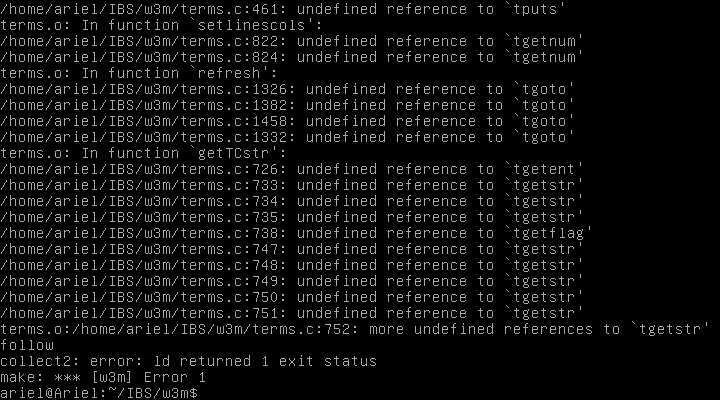
\includegraphics[width=.8\linewidth]{Images/Compile_w3m/libtinfo-dev_missing}
			\caption{Primer intento de ejecuci'on del makefile}
			\label{fig:libtinfo-dev_missing}
		\end{figure}
		
		El compilador no pudo encontrar las referencias de una serie de funciones utilizadas como \texttt{\textcolor{darkgray}{tputstring}} y otros con nombres similares. Luego de buscar un poco, averiguamos que 'estas podr'ian estar presentes en el paquete \texttt{libtinfo-dev}, el cual instalamos de la forma \texttt{sudo apt-get install libtinfo-dev}. Probamos nuevamente correr \texttt{make}.
		
		De todas formas, dada la rapidez con la que corri'o en comparaci'on a la anterior ejecuci'on, sumado a que se presentaron los mismos errores que dicha vez, probamos en cambio primero probar con correr \texttt{configure} otra vez, y luego \texttt{make}.
		
		%No había hecho captura cuando pensé que si :(
		%No pasa nada capo
		
		Comprobamos que el error antes experimentado desapareci'o, a cambio de otro nuevo:\enspace\verb|cannot stat `t-ja.gmo': No such file or directory|. Nuevamente investigamos este error y encontramos en un foro que un error id'entico se le present'o a un usuario cuando quiso instalar otro paquete\footnote{ \url{https://www.linuxquestions.org/questions/linux-general-1/alsa-utils-failing-make-stage-cannot-stat-\%60t-ja-gmo\%27-i-think-i-need-xgettext-386546/}}, y que se pod'ia resolver instalando el paquete \texttt{gettext}, de la forma \texttt{sudo apt-get install gettext}. Una vez instalado, al igual que antes, volvimos a correr \texttt{configure} y \texttt{make}.
		
		\begin{figure}[H]
			\centering \captionsetup{justification=centering}
			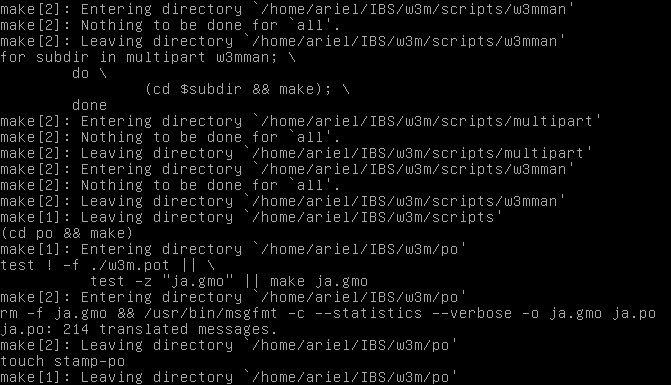
\includegraphics[width=.8\linewidth]{Images/Compile_w3m/make_successful}
			\caption{Segundo intento (y correcto) de ejecuci'on del makefile}
			\label{fig:make_successful}
		\end{figure}
		
		Esta vez no hubo ning'un error visible. Procedimos al paso final, a lo que corrimos \texttt{make install}.
		
		\begin{figure}[H]
			\centering \captionsetup{justification=centering}
			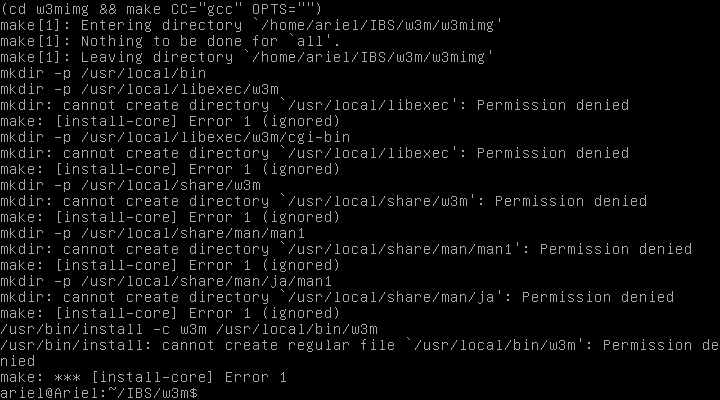
\includegraphics[width=.8\linewidth]{Images/Compile_w3m/make-install_fail}
			\caption{Primer intento fallido de ejecuci'on de \texttt{make install}}
			\label{fig:make-install_fail}
		\end{figure}
	
		Experimentamos una serie de \texttt{Permission denied}, y dedujimos que lo m'as probable era que, para correr este comando, requer'iamos de permisos root. Por lo tanto, probamos agregar \texttt{sudo}, al comienzo del comando.
		
		\begin{figure}[H]
			\centering \captionsetup{justification=centering}
			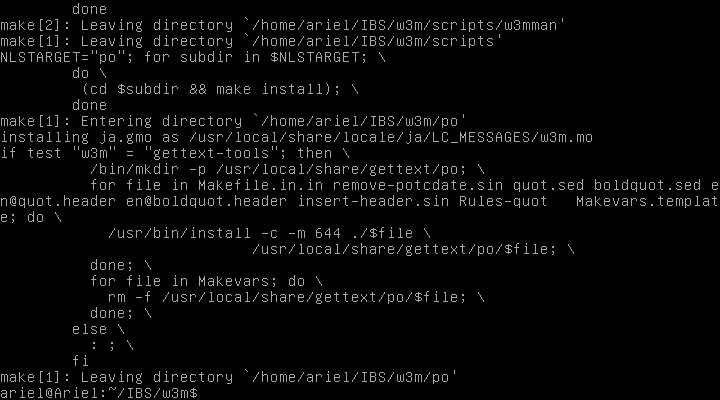
\includegraphics[width=.8\linewidth]{Images/Compile_w3m/make-install_successful}
			\caption{Segundo intento (y correcto) de ejecuci'on de \texttt{make install}}
			\label{fig:make-install_successful}
		\end{figure}
		
		Ning'un error visible. 'Este habr'ia sido el 'ultimo paso de la instalaci'on, y deber'iamos ser capaces de correr \texttt{w3m} correctamente. Para probar su funcionamiento, tratamos de entrar a \url{www.google.com} con el comando \texttt{w3m www.google.com}.
		
		\begin{figure}[H]
			\centering \captionsetup{justification=centering}
			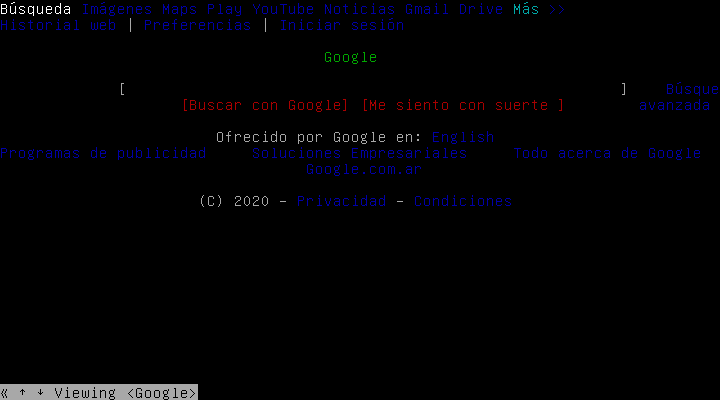
\includegraphics[width=.8\linewidth]{Images/Compile_w3m/test_w3m}
			\caption{Entrando a \url{www.google.com} con \texttt{w3m}}
			\label{fig:test_w3m}
		\end{figure}
		
		¡Y efectivamente pudimos visualizar el sitio web sin problemas! La compilaci'on de \texttt{w3m} fue exitosa.
		
		% Adoro los finales felices :D
		
	\section{Comandos usados}
		A continuaci'on se encuentran todos los comandos utilizados en este trabajo, correspondientes a las im'agenes presentadas.
		
		\begin{figure}[H]
			\centering
			\begin{code-box}
				\codetext{light-blue}{setlocal} \codetext{light-red}{number}
				
				\codetext{light-blue}{syntax} \codetext{light-red}{on}

				\codetext{light-blue}{colorscheme} \codetext{light-red}{desert}
				
				\codetext{light-blue}{setlocal} \codetext{light-red}{tabstop=4}

				\codetext{light-blue}{setlocal} \codetext{light-red}{shiftwidth=1}
				
				\codetext{light-blue}{setlocal} \codetext{light-red}{expandtab}
				
				\codetext{light-blue}{setlocal} \codetext{light-red}{softtabstop=4}
				
				\codetext{light-blue}{setlocal} \codetext{light-red}{autdoindent}
				
				\codetext{light-blue}{setlocal} \codetext{light-red}{smartindent}
			\end{code-box}
			\imagecaption{vim-setup}
		\end{figure}
		
		\begin{figure}[H]
			\centering
			\begin{code-box}
				\codetext{light-blue}{gcc} \codetext{orange-desert-vim}{-o circulo} \codetext{light-red}{circulo.c}
				
				\codetext{light-blue}{./circulo}
				
				\codetext{light-blue}{rm} \codetext{light-red}{circulo}
			\end{code-box}
			\imagecaption{basic-compilation}
		\end{figure}
		
		\begin{figure}[H]
			\centering
			\begin{code-box}
				\codetext{light-blue}{gcc} \codetext{orange-desert-vim}{-S} \codetext{light-red}{circulo.c}
				
				\codetext{light-blue}{head} \codetext{light-red}{circulo.s}
			\end{code-box}
			\imagecaption{complex-compilation}
		\end{figure}
		
		\begin{figure}[H]
			\centering
			\begin{code-box}
				\codetext{light-blue}{as} \codetext{orange-desert-vim}{-o circulo.o} \codetext{light-red}{circulo.s}
				
				\codetext{light-blue}{file} \codetext{light-red}{circulo.o}
			\end{code-box}
			\imagecaption{complex-assembly}
		\end{figure}
		
		\begin{figure}[H]
			\centering
			\begin{code-box}
			\codetext{light-blue}{ld} \codetext{orange-desert-vim}{-o circulo /usr/lib/gcc-lib/i386-linux/2.95.2/ collect2 -m elf\textunderscore{}i386 --dynamic-linker /lib/ld-linux.so.2 -o circulo /usr/lib/crt1.o /usr/lib/crti.o /usr/lib/gcc-lib/i386-linux/2.95.2/ crtbegin.o -L /usr/lib/gcc-lib/i386-linux/2.95.2} \codetext{light-red}{circulo.o }\codetext{orange-desert-vim}{-lgcc -lc -lgcc /usr/lib/gcc-lib/ i386-linux/2.95.2/crtend.o /usr/lib/crtn.o}
			\end{code-box}
			\imagecaption{first-ld-attempt}
		\end{figure}
		
		\begin{figure}[H]
			\centering
			\begin{code-box}
				\codetext{light-blue}{ld} \codetext{orange-desert-vim}{-o circulo} \codetext{light-red}{circulo.o} \codetext{orange-desert-vim}{-lc}
				
				\codetext{light-blue}{ld} \codetext{orange-desert-vim}{-o circulo} \codetext{light-red}{circulo.o} \codetext{orange-desert-vim}{-lc --entry main}
				
				\codetext{light-blue}{./circulo}
				
				\codetext{light-blue}{ld} \codetext{orange-desert-vim}{-l} \codetext{light-red}{circulo}
			\end{code-box}
			\imagecaption{second-ld-attempt}
		\end{figure}
		
		\begin{figure}[H]
			\centering
			\begin{code-box}
				\codetext{light-blue}{ld} \codetext{orange-desert-vim}{-o circulo -m elf\textunderscore\/i386 --dynamic-linker /lib/ld-linux.so.2} \codetext{light-red}{circulo.o} \codetext{orange-desert-vim}{-lc --entry main}
				
				\codetext{light-blue}{./circulo}
				
				\codetext{light-blue}{gdb} \codetext{light-red}{circulo}
				
				\codetext{light-green}{(gdb)} \codetext{light-blue}{r}
			\end{code-box}
			\imagecaption{third-ld-attempt}
		\end{figure}
		
		\begin{figure}[H]
			\centering
			\begin{code-box}
				\codetext{light-blue}{ld }\codetext{orange-desert-vim}{-o circulo -m elf\textunderscore\/i386 --dynamic-linker /lib/ld-linux.so.2 /usr/lib/i386-linux-gnu/ crt1.o /usr/lib/i386-linux-gnu/crti.o} \codetext{light-red}{circulo.o} \codetext{orange-desert-vim}{-lc /usr/lib/i386-linux-gnu/crtn.o}
				
				\codetext{light-blue}{./circulo}
			\end{code-box}
			\imagecaption{fourth-ld-attempt}
		\end{figure}
		
		%%%%%%
		\begin{figure}[H]
			\centering
			\begin{code-box}
			    	\codetext{light-blue}{gcc }\codetext{orange-desert-vim}{--static -o circulo\_estatico }\codetext{light-red}{circulo.c}
                
                		\codetext{light-blue}{./circulo\_estatico}\newline
                	
                		\codetext{light-blue}{gcc }\codetext{orange-desert-vim}{-o circulo\_dinamico }\codetext{light-red}{circulo.c}
                
               			 \codetext{light-blue}{./circulo\_dinamico}
			\end{code-box}
			\imagecaption{andan}
		\end{figure}
		
    		\begin{figure}[H]
			\centering
			\begin{code-box}
			 	\codetext{light-blue}{file }\codetext{light-red}{circulo\_estatico}
    
               			\codetext{light-blue}{file }\codetext{light-red}{circulo\_dinamico}
                
			\end{code-box}
			\imagecaption{bien_enlazados}
		\end{figure}
		
	   	 \begin{figure}[H]
			\centering
			\begin{code-box}
				\codetext{light-blue}{ls }\codetext{orange-desert-vim}{-l }\codetext{light-red}{circulo\_estatico circulo\_dinamico}
            		\end{code-box}
			\imagecaption{bytes_circulos}
		\end{figure}
	
    		\begin{figure}[H]
			\centering
			\begin{code-box}
				\codetext{light-blue}{gcc }\codetext{orange-desert-vim}{--static -o cos\_estaticas }\codetext{light-red}{cosas\_innecesarias.c}
        
                  		\codetext{light-blue}{file }\codetext{light-red}{cos\_estaticas}\newline
    
                		\codetext{light-blue}{gcc }\codetext{orange-desert-vim}{-o cos\_dinamicas }\codetext{light-red}{cosas\_innecesarias.c}

                		\codetext{light-blue}{file }\codetext{light-red}{cos\_dinamicas}
			\end{code-box}
			\imagecaption{innecesario}
		\end{figure}
    
    		\begin{figure}[H]
			\centering
			\begin{code-box}
				\codetext{light-blue}{./cos\_estaticas}
			    
                		\qquad\codetext{orange-desert-vim}{[Ctrl + Z]}\newline
                
                		\codetext{light-blue}{./cos\_dinamicas}
                
                 		\qquad\codetext{orange-desert-vim}{[Ctrl + Z]}
			\end{code-box}
			\imagecaption{detenidos}
		\end{figure}

     		\begin{figure}[H]
        		\centering
        		\begin{code-box}
            			\codetext{light-blue}{ps }\codetext{orange-desert-vim}{auxT}
        		\end{code-box}
        	\imagecaption{ps}
    		\end{figure}
		
		\begin{figure}[H]
			\centering
			\begin{code-box}
				\codetext{light-blue}{wget} \codetext{orange-desert-vim}{-q -O calc.h} \codetext{light-red}{iie.fing.edu.uy/\textasciitilde{}vagonbar/gcc-make/ polaca/calc.h}
				
				\codetext{light-blue}{wget} \codetext{orange-desert-vim}{-q -O getch.c} \codetext{light-red}{iie.fing.edu.uy/\textasciitilde{}vagonbar/gcc-make/ polaca/getch.c}
				
			  	\codetext{light-blue}{wget} \codetext{orange-desert-vim}{-q -O getop.c} \codetext{light-red}{iie.fing.edu.uy/\textasciitilde{}vagonbar/gcc-make/ polaca/getop.c}
				
				\codetext{light-blue}{wget} \codetext{orange-desert-vim}{-q -O  main.c} \codetext{light-red}{iie.fing.edu.uy/\textasciitilde{}vagonbar/gcc-make/ polaca/main.c}
				
				\codetext{light-blue}{wget }\codetext{orange-desert-vim}{-q -O stack.c} \codetext{light-red}{iie.fing.edu.uy/\textasciitilde{}vagonbar/gcc-make/ polaca/stack.c}
			
			\end{code-box}
			\imagecaption{makefile-download}
		\end{figure}
		
		\begin{figure}[H]
			\centering
			\begin{code-box}
				\codetext{light-blue}{gcc }\codetext{orange-desert-vim}{-o main }\codetext{light-red}{main.c getch.c getop.c stack.c}
			\end{code-box}
			\imagecaption{makefile-gcc-compile}
		\end{figure}
		
		\begin{figure}[H]
			\centering
			\begin{code-box}
				\codetext{light-blue}{make } \codetext{light-red}{polaca}
                
                		\codetext{light-blue}{make } \codetext{light-red}{clean}

			\end{code-box}
			\imagecaption{makefile-successful-compile}
		\end{figure}
		
		\begin{figure}[H]
			\centering
			\begin{code-box}
				\codetext{light-blue}{./configure}

			\end{code-box}
			\imagecaption{g++_missing}
		\end{figure}
		
		%g++_missing_log, creo que no es necesario copiar nada acá
		%gc_missing, lo mismo
		%libtinfo-dev_missing, lo mismo
		
	    	\begin{figure}[H]
			\centering
			\begin{code-box}
			    \codetext{light-blue}{sudo apt-get }\codetext{orange-desert-vim}{install }\codetext{light-red}{gettext}

				\codetext{light-blue}{./configure}

				\codetext{light-blue}{make}

			\end{code-box}
			\imagecaption{make_successful}
		\end{figure}
		
		 \begin{figure}[H]
			\centering
			\begin{code-box}
			    \codetext{light-blue}{make }\codetext{orange-desert-vim}{install}
			\end{code-box}
			\imagecaption{make-install_fail}
		\end{figure}
		
		\begin{figure}[H]
			\centering
			\begin{code-box}
			    \codetext{light-blue}{sudo make }\codetext{orange-desert-vim}{install}
			\end{code-box}
			\imagecaption{make-install_successful}
		\end{figure} 

		\begin{figure}[H]
			\centering
			\begin{code-box}
			    \codetext{light-blue}{w3m} \codetext{light-red}{www.google.com}
			\end{code-box}
			\imagecaption{test_w3m}
		\end{figure} 

	\section{Archivos generados}
		 A continuaci'on se encuentran todos los archivos que creamos para hacer este trabajo, correspondientes a las im'agenes presentadas.

		\lstset{style=mystyle}
		\lstinputlisting[language=C, title=\char91\ref{fig:circle-code}\char93\:{}Archivo \texttt{circulo.c}]{archivos/circulo.c}
		
		\lstinputlisting[language=C, title=\char91\ref{cosas_innecesarias}\char93\:{}Archivo \texttt{cosas\_innecesarias.c}]{archivos/cosas_innecesarias.c}
		
		\lstinputlisting[language=make, title=\char91\ref{fig:makefile}\char93\:{}Makefile de \texttt{polaca}.]{archivos/makefile_pol.txt}
		
		
		
		
		
		
		
				

		


















%Remove whitspace when done, for ease of work.
\end{document}
